% RCLN manuscript -- English version for Nature Communications (v3, 2026-08-14)
% Compile with pdflatex (no CJK dependency). All numbers trace to results/paper_experiments/ JSONs.
% Official-template switch: replace the documentclass/preamble block with
%   \documentclass[pdflatex,sn-nature]{sn-jnl}
% (sn-jnl is preloaded in the Overleaf "Springer Nature" gallery template); see README.md.
\documentclass[11pt,a4paper]{article}
\usepackage[a4paper,margin=2.4cm]{geometry}
\usepackage{amsmath,amssymb,amsthm,bm}
\usepackage{booktabs,array,multirow,tabularx}
\usepackage{graphicx}
\usepackage{xcolor}
\usepackage{enumitem}
\usepackage{caption}
\usepackage[super,sort&compress]{cite}
\usepackage[hidelinks]{hyperref}
\captionsetup{font=small,labelfont=bf}
\newtheorem{theorem}{Theorem}
\newtheorem{corollary}{Corollary}
\newtheorem{definition}{Definition}
\newtheorem{remark}{Remark}
\newcommand{\bu}{\bm{u}}
\newcommand{\cF}{\mathcal{F}}
\newcommand{\cC}{\mathcal{C}}
\newcommand{\cH}{\mathcal{H}}
\newcommand{\cS}{\mathcal{S}}
\newcommand{\cX}{\mathcal{X}}
\newcommand{\Ex}{E}
\newcommand{\inner}[2]{\langle #1, #2 \rangle}

\title{\bfseries Architecture-embedded physical constraints enable stable\\ long-horizon neural PDE prediction}
% TODO(user): fill in affiliation and the corresponding email before submission.
\author{Yuze Chen$^{1,*}$\\[4pt]
\normalsize $^{1}$[Department, University, City, Country]\\
\normalsize $^{*}$Corresponding author: [email]}
\date{}

\begin{document}
\maketitle

\begin{abstract}
\noindent Neural operators now predict the short-term evolution of partial differential equations with high fidelity, but long-horizon autoregressive rollout remains unstable: errors compound over hundreds of steps and end in energy blow-up or field collapse. Here we argue that this fragility is structural---physical knowledge is placed where it can be bypassed. As a soft penalty in the training loss, physics is a suggestion; as post-processing after the network, it is a patch; neither prevents a network from leaving the physically feasible set at inference. We propose architecture-level physical anchoring: exactly known dynamics---conservation projections, exact linear propagators and dissipation envelopes---are hard-coded as zero-parameter operators inside the forward pass, while data-driven modules learn only the unresolved residual under geometric gating. Under one retrained, controlled protocol across three mechanistically distinct systems---3D decaying turbulence, 2D forced turbulence and 1D chaos---the anchored model completes 200-step rollouts with zero crashes and a 1.1\% energy bias, whereas mainstream baselines retrained under the same protocol all fail. The same constraints prevent blow-up across systems and resolutions without recalibration, while loss-level physics consistently fails. Where physics is embedded determines the stability properties of neural PDE prediction.
\end{abstract}

\noindent\textbf{Keywords}: physics-informed machine learning; neural operators; long-horizon stability; constraint-preserving architectures; error diagnosis

\section*{Introduction}

In scientific machine learning, \emph{where} physical knowledge is embedded determines what it can achieve. Inserted into the training objective as a soft penalty, physics is a \emph{suggestion}: once training ends, nothing prevents the model from violating it at inference. Applied after the network as projection or rescaling, physics is a \emph{patch}: the network never sees its own corrected outputs, and errors compound between the two stages. Embedded as a structural component of the inference path---an architectural prior---physics becomes \emph{law}: every rollout step lands inside the physically feasible set by construction. In this work we show that for long-horizon autoregressive PDE prediction, only the third position changes the stability properties of the learned dynamics.

The question is urgent because of a widening gap. Neural operators---Fourier neural operators\cite{li2021fno}, U-Nets\cite{ronneberger2015}, DeepONets\cite{lu2021deeponet} and transformer-based solvers\cite{hao2024dpot,wu2024transolver}---now approach the fine-scale dynamics of viscous flows over one or a few steps\cite{kovachki2023,azizzadenesheli2024}, and data-driven models have reached remarkable skill in weather and climate prediction\cite{lam2023graphcast,kochkov2024neuralgcm}. Yet long-horizon rollout, in which the model feeds on its own outputs for hundreds of steps, still fails almost universally\cite{brandstetter2022mpnpde,mccabe2023stability}; diffusion-based refinement restores long rollouts only at heavy per-step cost\cite{lippe2023pderefiner}, and stable hybrid ML--CFD couplings succeed by engineering the coupling, not by trusting the network\cite{kochkov2021mlcfd}. Failure has two faces: energy blow-up (numerical instability) and over-dissipation (the field regresses toward the training mean and turbulent structures die). The second is more insidious: the model does not crash, but it is already physically wrong. We will show that both failures share one root cause, and admit one prescription.

This work makes three contributions. (i) \textbf{A transferable methodological principle}: physics should be enforced on the inference path rather than encouraged in the training loss. We reproduce the superiority of architectural anchoring over loss-level physics under a fully isomorphic controlled protocol on three mechanistically distinct systems: 3D incompressible decaying turbulence (conservation-law physics), 2D forced Kolmogorov turbulence (linear-operator plus hypofriction physics) and the 1D chaotic Kuramoto--Sivashinsky equation (dispersion--dissipation physics). The three systems are chosen deliberately: they cover conservation laws, linear operators and dissipation inequalities---the three families of physics that can be hard-coded exactly---and their chaotic and turbulent characters differ, forming a minimal sufficient test of generality. (ii) \textbf{Deterministic theoretical guarantees}: theorems on divergence-free output, dissipation compatibility and bounded correction, plus a finite-horizon boundedness corollary (Section~\ref{sec:theory}), whose proofs never invoke any internal property of the neural network. (iii) \textbf{An emergent error-diagnosis signal}: the geometric discrepancy between anchor and residual predicts where the prediction will go wrong (AUROC $0.786$) with no error labels, no additional parameters and no extra forward passes, and transfers zero-shot to a frozen backbone ($0.805$).

\textbf{Relation to prior work}. The neural-operator lineage (FNO, U-Net, DPOT, Transolver and successors) has improved one-step accuracy, but our fair benchmark (Results) shows that their long-horizon failure modes differ---blow-up, over-dissipation, insufficient accuracy---indicating an architecture-level problem shared across families\cite{li2021fno,ronneberger2015,hao2024dpot,wu2024transolver}. Physics-informed training (the PINN/PINO lineage\cite{raissi2019pinn,li2024pino}) imposes equation residuals as soft penalties and is highly effective for forward and inverse problems\cite{karniadakis2021,wang2021pideeponet}, but soft constraints do not prevent autoregressive drift; the failure of our loss-level arm is direct controlled evidence. Post-hoc stabilisation places physics outside the network---for example, projecting each prediction onto the PDE-consistent manifold\cite{huang2025physicorrect}---and we find this two-stage structure systematically inferior to joint training at long horizon (Table~\ref{tab:ablation}). Hard-constraint designs exist---exact conservation in latent dynamics\cite{lee2021deepconservation}, hard constraints in turbulence coarse-graining\cite{mohan2023hard}, and hard-constraint scaling with mixture-of-experts\cite{chalapathi2024moe}---but they target single-system accuracy rather than the position question posed here. Structure-preserving numerical methods (geometric integration, projection methods, limiters\cite{hairer2006gni,chorin1968}) are theoretically complete in classical numerical analysis; our principle can be read as their architecture-level realisation inside a learnable simulator (Discussion; Supplementary Information SI-B). Hybrid physics--network augmentation\cite{yin2021aphynity} shares our residual philosophy but leaves the learned component unconstrained. Uncertainty quantification (MC-dropout\cite{gal2016dropout}, deep ensembles\cite{lakshminarayanan2017}) requires multiple stochastic forward passes; our discrepancy signal costs zero extra passes, and we deliberately name it a discrepancy indicator rather than an uncertainty estimator (Results). Within this journal, stable machine-learning parameterisation\cite{yuval2020stable} and latent-space operator learning\cite{kontolati2024latent} have shown that placing physics inside the computation graph pays off; the present work isolates the position principle itself and tests it under controlled, retrained comparisons.

\section{Results}

\subsection{Architecture: physics on the inference path}\label{sec:arch}

\textbf{Problem setup}. Given a state $\bu_t\in\cX\subset L^2(\Omega)^d$ on a periodic domain $\Omega$, a one-step propagator $\cF_\theta:\cX\to\cX$ generates a long-horizon trajectory autoregressively,
\begin{equation}
\bu_{t+1}=\cF_\theta(\bu_t),\qquad t=0,1,\dots,K-1 .
\label{eq:rollout}
\end{equation}
Chaotic and turbulent systems have positive Lyapunov exponents, so one-step errors are amplified by $e^{\lambda_{\max}\Delta t}$ per step; at $K\sim O(10^2)$, any one-step accuracy advantage is dominated by stability. The goal is to construct $\cF_\theta$ such that the trajectory remains inside the physically feasible set for the entire horizon while preserving correct statistical physics.

\begin{definition}[Physically feasible set]
For 3D incompressible decaying flow,
\begin{equation}
\cC_{\mathrm{phys}}=\Big\{\bu:\ \nabla\!\cdot\!\bu=0,\quad \Ex(\bu_{\mathrm{in}})-c_d\,\varepsilon(\bu_{\mathrm{in}})\,\Delta t\le \Ex(\bu)\le \Ex(\bu_{\mathrm{in}})\Big\},
\label{eq:feasible}
\end{equation}
where $\Ex(\bu)=\tfrac12\langle\|\bu\|^2\rangle_\Omega$ is the kinetic-energy density, $\varepsilon(\bu)=\nu\langle\|\nabla\times\bu\|^2\rangle_\Omega$ the enstrophy dissipation rate, and $c_d>1$ a calibrated dissipation constant. For driven systems (2D forced turbulence, KS), the no-growth ceiling is replaced by a production-rate bound (Eq.~\eqref{eq:env-driven}).
\end{definition}

The three elements encode a kinematic constraint (zero divergence), a thermodynamic direction (energy cannot increase) and a bound on the dissipation rate. This differs essentially from our earlier projection that pulled the energy back to the input value at every step: at finite Reynolds number the true solution necessarily dissipates, and $\Ex/\Ex_0\equiv1$ is the wrong physics.

\textbf{Physical anchor: zero-parameter carriers of exactly known dynamics}. \emph{3D incompressible flow: the Leray projection.} On a periodic domain the Helmholtz--Leray decomposition is the spectral projection
\begin{equation}
\widehat{\bu}_{\mathrm{sol}}(\bm{k})=\Big(\bm{I}-\frac{\bm{k}\bm{k}^{\mathsf T}}{\|\bm{k}\|^2}\Big)\widehat{\tilde\bu}(\bm{k}),\qquad \bm{k}\neq\bm{0},
\label{eq:leray}
\end{equation}
leaving the zero mode unchanged. The projection is idempotent, orthogonal, parameter-free and differentiable inside the forward pass of $\cF_\theta$.

\emph{Exact linear propagators (2D/1D).} The 1D Kuramoto--Sivashinsky equation\cite{kuramoto1976,sivashinsky1977} $u_t=-uu_x-u_{xx}-u_{xxxx}$ has the linear symbol
\begin{equation}
\lambda(k)=k^2-k^4,\qquad k=\tfrac{2\pi n}{L},
\label{eq:ks-symbol}
\end{equation}
unstable at low wavenumbers and strongly dissipative at high ones. The 2D vorticity--stream-function form $\omega_t+J(\psi,\omega)=\nu\Delta\omega+f_\omega-\alpha\Delta^{-1}\omega$ (with $\hat\psi=-\hat\omega/\|\bm{k}\|^2$, $\bu=\nabla^\perp\psi$) has the linear symbol
\begin{equation}
\lambda(\bm{k})=-\nu\|\bm{k}\|^2-\alpha\|\bm{k}\|^{-2},
\label{eq:ns2d-symbol}
\end{equation}
where $\alpha\Delta^{-1}\omega$ is the hypofriction that suppresses the 2D inverse-cascade pile-up. Stationary forcing is integrated exactly with the $\varphi_1$ function:
\begin{equation}
\widehat{\omega}_{t+1}=e^{\lambda(\bm{k})\Delta t}\widehat{\omega}_t+\varphi_1\!\big(\lambda(\bm{k})\Delta t\big)\,\Delta t\,\widehat f_\omega,\qquad \varphi_1(z)=\frac{e^{z}-1}{z}.
\label{eq:phi1}
\end{equation}
Equation~\eqref{eq:phi1} matches the linear propagator of the data generator (contour-integral ETDRK4\cite{cox2002etdrk4,kassam2005}) term by term (numerically verified, maximal error $3\times10^{-8}$). In the vorticity--stream-function representation the divergence-free identity holds automatically; no extra projection is needed.

\textbf{Dissipation-aware energy envelope}\label{sec:envelope}. For \emph{decaying flows} (3D TGV, 2D decaying), the per-step admissible interval is strict:
\begin{equation}
\Ex(\bu_{t+1})\in\big[\Ex(\bu_t)-c_d\,\varepsilon(\bu_t)\,\Delta t,\ \Ex(\bu_t)\big]\qquad(\text{decay, strict}).
\label{eq:env-decay}
\end{equation}
A relaxed no-growth rule with slack $\gamma>0$ does not survive compounding ($\gamma=0.005$ amplifies $2.7\times$ over 200 steps), so we adopt the strict form. For \emph{driven systems} (2D Kolmogorov, KS) the energy can rebound, and we use a two-sided rate envelope instead:
\begin{equation}
\Ex(\bu_{t+1})\in\big[\Ex(\bu_t)-c_d\,D(\bu_t)\Delta t,\ \Ex(\bu_t)+c_p\,P(\bu_t)\Delta t\big],
\label{eq:env-driven}
\end{equation}
with $P,D$ the known production and dissipation rates (identities in Section~\ref{sec:theory}). Out-of-bound outputs receive a minimal intervention---a uniform rescaling
\begin{equation}
\bu_{t+1}\leftarrow \alpha\,\bu_{t+1}^{\mathrm{pred}},\qquad \alpha=\sqrt{\Ex_{\mathrm{bound}}/\Ex(\bu_{t+1}^{\mathrm{pred}})},
\label{eq:rescale}
\end{equation}
and the hit rate together with the mean correction $|\alpha-1|$ is logged exhaustively. The calibration protocol is uniform across systems: the $p_{99.5}$ quantile of the training-trajectory ratio $\Delta\Ex/(\mathrm{rate}\cdot\Delta t)$, multiplied by a safety factor of $1.2$.

\textbf{Soft residual learner and geometric gating}. The residual learner $\cS_\phi$ learns only the increments the anchor leaves unresolved. Fusion is driven by per-voxel error radii $\hat e_g,\hat e_l$ estimated by a calibration head:
\begin{equation}
w(\bm{x})=\frac{\hat e_g(\bm{x})^{\beta}}{\hat e_g(\bm{x})^{\beta}+\hat e_l(\bm{x})^{\beta}},\qquad
R_{\mathrm{eff}}=\max\!\big(1.54\,\hat e_g(\bm{x}),\ 0.05\big),
\label{eq:gate}
\end{equation}
\begin{equation}
\bu_{\mathrm{fused}}=(1-w)\,\bu_{\mathrm{anchor}}+w\,\bu_{\mathrm{soft}},\qquad
\text{s.t.}\ \|\bu_{\mathrm{fused}}-\bu_{\mathrm{anchor}}\|_{\cX}\le R_{\mathrm{eff}} .
\label{eq:fusion}
\end{equation}
The gating signal $s(\bm{x},t)$ is additionally exported as the discrepancy indicator (Section~\ref{sec:upi}).

\textbf{Why this is not ``an FNO with hard constraints''}. The three components have legible, disjoint roles: the anchor answers \emph{what does the known physics allow} (run alone, its energy stays near the truth but rL2 $>1.5$---feasibility without accuracy); the residual learner answers \emph{what does the known physics fail to explain} (run alone, its energy drifts to $2.9\times$---free correction necessarily leaves the feasible set); the geometry gate answers \emph{how much correction is each step allowed}. Removing any single component destroys the main result (zero crashes with $1.1\%$ energy bias; Table~\ref{tab:ablation}). Components of a modular stack can be deleted one by one without fatal damage; ours cannot---that is the criterion distinguishing architecture design from stacking. Moreover, the constraints participate in the forward pass and in back-propagation: the residual learner is trained directly to predict \emph{along the boundary of the feasible set}, which is structurally different from any post-processing pipeline.

\textbf{Training objective}. A multi-step curriculum loss with scheduled sampling:
\begin{equation}
\mathcal{L}=\sum_{k=0}^{R-1}\gamma_r^{k}\,\big\|\cF_\theta^{(k)}(\bu_t)-\bu_{t+k+1}\big\|^2,\qquad R=3,\ \gamma_r=0.9 .
\label{eq:loss}
\end{equation}
The loss contains \textbf{no} physical penalty term---physics is carried entirely by the architecture. This is the only difference from the loss-level arm, and constitutes the controlled contrast.

\subsection{Theoretical guarantees}\label{sec:theory}

We state deterministic conclusions that hold without observing the ground truth (full proofs in SI-A). We deliberately drop the optimality claim of an earlier draft---``the fused output is no worse than the better of the two branches''---because it does not follow from geometric gating; the theoretical goal shifts from \emph{who is more accurate} to \emph{why the trajectory cannot leave the feasible set}.

\begin{theorem}[Divergence-free output]\label{thm:div}
Suppose $\cH$ contains the Leray projection~\eqref{eq:leray} and every step's correction exits through the projection. Then for any input, the rollout output satisfies $\nabla\!\cdot\!\bu_{t+1}=0$ (to spectral accuracy).
\end{theorem}
\begin{proof}[Proof idea]
By idempotency of the projection and the equivalence of $\bm{k}\cdot\widehat{\bu}=0$ in Fourier space (SI-A).
\end{proof}

\begin{theorem}[Dissipation compatibility]\label{thm:energy}
With the envelope~\eqref{eq:env-decay}--\eqref{eq:rescale} active, every step's output energy in decaying flow falls exactly inside the admissible interval; the energy sequence is non-increasing and bounded below, hence convergent.
\end{theorem}
\begin{proof}[Proof idea]
The scalar scaling identity $\Ex(\alpha\bu)=\alpha^2\Ex(\bu)$ plus the monotone convergence principle (SI-A).
\end{proof}

\begin{theorem}[Bounded correction / soft landing]\label{thm:gate}
The fused output deviates from the anchor by at most $\|\bu_{\mathrm{fused}}-\bu_{\mathrm{anchor}}\|\le R_{\mathrm{eff}}$ uniformly; at initialisation the gate tightens automatically ($\lambda<1$) and relaxes as the residual learner's violation production decays ($\lambda\to1$).
\end{theorem}
\begin{proof}[Proof idea]
Spherical-projection construction and monotonicity of the contraction factor $\lambda=\exp(-\Sigma/\tau)$ (SI-A).
\end{proof}

\begin{corollary}[Finite-horizon rollout boundedness]\label{cor:bounded}
If the residual learner is Lipschitz (structurally maintained by spectral normalisation) and the anchor is non-expansive, then any $K$-step trajectory is stepwise divergence-free, energy-feasible and uniformly norm-bounded: blow-up divergence is excluded by construction.
\end{corollary}

\begin{remark}
Theorem~\ref{thm:energy} guarantees \emph{feasibility}, not \emph{accuracy}: the envelope does not force dissipation to occur on schedule (the measured $\varepsilon(t)$ shows a delayed-release profile, reported honestly in Section~\ref{sec:fidelity}). This is precisely why the theoretical target moved from optimality to feasibility.
\end{remark}

\textbf{Energy budget identities (the physical basis of the envelopes)}. The envelope boundaries are fixed by the exact energy identity of each equation. For \textbf{KS}, multiplying $u_t=-uu_x-u_{xx}-u_{xxxx}$ by $u$ and averaging over the periodic domain kills the nonlinear term by parts, giving
\begin{equation}
\frac{\mathrm{d}\Ex}{\mathrm{d}t}=\underbrace{\langle u_x^2\rangle}_{P\ (\text{production})}-\underbrace{\langle u_{xx}^2\rangle}_{D\ (\text{dissipation})},\qquad \Ex=\tfrac12\langle u^2\rangle .
\label{eq:ks-budget}
\end{equation}
For \textbf{2D NS in vorticity form}, the Jacobian term conserves energy and
\begin{equation}
\frac{\mathrm{d}\Ex}{\mathrm{d}t}=-2\nu Z+\inner{\bu}{\bm f}-2\alpha\Ex_{\mathrm{low}},\qquad
\frac{\mathrm{d}Z}{\mathrm{d}t}=-\nu\langle\|\nabla\omega\|^2\rangle+\langle\omega f_\omega\rangle-\alpha(\text{low-mode term}),
\label{eq:ns2d-budget}
\end{equation}
where $Z=\tfrac12\langle\omega^2\rangle$ is the enstrophy. In decaying flow ($\bm f{=}0,\alpha{=}0$) energy and enstrophy both decay monotonically---2D offers one more hard constraint than 3D, which we exploit as a diagnostic. For \textbf{3D incompressible NS}, $\mathrm{d}\Ex/\mathrm{d}t=-\varepsilon(\bu)$, the physical source of Eq.~\eqref{eq:env-decay}; the calibration constant absorbs discretisation and unresolved subgrid dissipation (truth ratio $p_{99.5}=1.015$, times safety factor $1.2$, giving $1.218$).

\subsection{A controlled protocol for long-horizon comparison}\label{sec:setup}

Fair comparison is itself part of the methodology. \textbf{Every compared model is retrained under an identical protocol}: same data split, same training budget, same optimiser, same rollout curriculum---the only experimental variable is \emph{where the physics is placed}. Three arms per system: (i) \textbf{anchor}: architecture-level physics (anchor $+$ envelope $+$ gate); (ii) \textbf{loss-level}: the same network trained with $\mathcal{L}_{\mathrm{MSE}}+0.1\,\mathcal{L}_{\mathrm{PDE\ residual}}$; (iii) \textbf{none}: purely data-driven. Parameter counts are strictly matched (3D $5.10$M; 2D $1.19$M; 1D $0.29$M; the anchor adds zero parameters). External baselines---FNO (official implementation\cite{kossaifi2024library}), DPOT, U-Net, FNO with physics regularisation---are retrained under the same protocol as the 3D backbone; PhysicsCorrect\cite{huang2025physicorrect}, whose official code is unavailable, is approximately reproduced and labelled as such; Transolver diverged under the same protocol (its fp32 fallback also exceeded the pre-set time budget) and was abandoned by a pre-registered rule, with DPOT satisfying the ``at least one recent method'' requirement. Datasets, generators and verification discipline are detailed in Methods; the crash criteria are given in Table~\ref{tab:crash}. A claim of ``zero crashes'' is meaningful only under strict criteria: a previous internal baseline line reported zero crashes under a lenient rL2${}>10$ threshold, where a one-sided $1.05\times$ anti-blow-up net compounded over 200 steps into an effective $1.7\times10^{4}$ energy ceiling---no constraint at all.

\begin{table}[htbp]
\centering\small
\caption{\textbf{Crash criteria and rationale}. Post-crash metrics are frozen-filled to step $K$ to avoid survivorship bias.}
\label{tab:crash}
\begin{tabular}{lll}
\toprule
Criterion & Threshold & Rationale \\
\midrule
Non-finite value & NaN/Inf & Numerical blow-up \\
Relative $L_2$ error & $>5$ & Field corruption \\
Energy ratio $E/E_0$ & $>5$ & Energy explosion \\
Post-crash handling & Frozen filling & Avoids survivorship bias \\
\bottomrule
\end{tabular}
\end{table}

\textbf{Evaluation conventions}. rL2 is computed in physical space (after de-normalisation); $K\in\{1,10,50,100,200\}$; 10 ICs on the main system, 5 ICs in-domain for 2D, 3 ICs for OOD; envelope interventions are logged exhaustively; every long-horizon comparison reports the triple (rL2, $E/E_0$, crash rate); per-IC raw curves are released with the code.

\subsection{Main benchmark: divergent long-horizon fates from one initial condition}\label{sec:main}

Figure~\ref{fig:fig1} contrasts the two paradigms (bypassable vs non-bypassable constraints) and shows the long-horizon fate bifurcation from a single initial condition: the official FNO blows up at $k\approx131$, the physics-regularised FNO at $k\approx99$, while our model tracks the true energy trajectory throughout (the logarithmic inset shows the complete runaway before the first crash).

\begin{figure}[htbp]
\centering
\includegraphics[width=\textwidth]{figures/fig1_concept_failure.pdf}
\caption{\textbf{Concept and failure modes}. (a) In the predict-then-correct paradigm the physical constraint can be bypassed. (b) Our architecture: physical anchor $\to$ residual learning $\to$ geometric gating; the constraint sits on the inference path and cannot be bypassed (blue $=$ anchor, green $=$ residual, orange $=$ gate). (c) Long-horizon energy trajectories from one initial condition: our model (red) tracks the truth (dashed), while the FNO-family baselines blow up in turn; the inset shows the full runaway on a logarithmic axis ($\times$ marks the first crash). Post-crash states are non-finite; curves are held at their last finite value for display.}
\label{fig:fig1}
\end{figure}

\begin{table}[htbp]
\centering\small
\caption{\textbf{Main long-horizon benchmark} (3D TGV, Re$=6400$, $K{=}200$, 10 initial conditions, mean$\pm$std). Truth: $E/E_0$ at $K{=}200$ is $0.9416$. All models are retrained under the identical protocol (Section~\ref{sec:setup}); the only experimental variable is where the physics is placed.}
\label{tab:main}
\setlength{\tabcolsep}{3pt}
\begin{tabular}{@{}lccccccc@{}}
\toprule
Model & Params & rL2@50 & rL2@100 & rL2@200 & $E/E_0$@200 & Crashes & ms/step \\
\midrule
\textbf{RCLN (ours)} & 5.10M & $\bm{0.2554}$ & $\bm{0.4670}$ & $1.0237$ & $\bm{0.9314\pm0.0027}$ & $\bm{0/10}$ & 64.5 \\
FNO (official) & 6.70M & $0.1857$ & $0.8946$ & $2.1653$ & $5.0930$ & $10/10$ & 58.5 \\
U-Net & 6.32M & $0.3499$ & $0.7638$ & $1.2001$ & $0.6674$ & $0/10$ & 35.2 \\
DPOT (recent) & 10.82M & $1.1104$ & $1.4051$ & $1.4569$ & $1.5174$ & $0/10$ & 15.5 \\
FNO$+$PhysReg & 6.70M & $0.3889$ & $2.1803$ & $2.1938$ & $5.1066$ & $10/10$ & 58.1 \\
PhysicsCorrect (approx.) & 6.70M & $0.2729$ & $0.5372$ & $1.0986$ & $1.1792$ & $0/10$ & 60.7 \\
\bottomrule
\end{tabular}
\end{table}

\textbf{Energy fidelity}: ours reaches $E/E_0=0.9314\pm0.0027$ at $K{=}200$ ($1.1\%$ bias from truth; maximal pointwise deviation $1.0\%$; the no-envelope backbone deviates by $14.7\%$)---the only model that neither amplifies energy (FNO family: $5.1\times$ explosion) nor over-dissipates (U-Net: $0.667$). \textbf{Accuracy}: ours is best at rL2@50 and rL2@100; FNO is more accurate short-term (rL2@50 $=0.186$) but crashes at $k=126$--$133$ in $10/10$ trajectories. \textbf{Error-growth dynamics}: the ten first-crash steps of FNO, $\{133,133,133,133,133,132,130,129,128,126\}$, are tightly clustered---not gradual degradation but threshold-crossing blow-up, consistent with the mechanism ``missing constraint $\to$ high-wavenumber energy pile-up $\to$ aliasing instability''. Our model's rL2$(k)$ grows as a power law up to $k\le100$ and then enters a decorrelation plateau; envelope interventions split about evenly between floor and ceil with a mean correction of $1.9\%$---mild and two-sided. U-Net deserves a separate note: zero crashes and rL2@200 $=1.20$ look robust, but its energy falls to $66.7\%$---its ``stability'' is bought by dissipating itself into a low-energy state, visible only if the energy budget is reported. \textbf{Cost}: $+8.6\%$ single-step inference time ($59.4\to64.5$ ms), zero extra parameters.

\begin{figure}[htbp]
\centering
\includegraphics[width=\textwidth]{figures/fig3_tgv_main.pdf}
\caption{\textbf{Main 3D TGV results} (Re$=6400$, 10 ICs). (a) rL2$(k)$ with standard-deviation band. (b) Survival curves (vertical dashed lines mark first-crash steps: FNO $k{\approx}131$, FNO$+$PhysReg $k{\approx}99$). (c) Energy trajectory $E(t)$ against truth; the grey band is the stepwise physically feasible interval of Theorem~\ref{thm:energy} (inset: zoom of $k{=}150$--$200$). (d) Dissipation rate $\varepsilon(t)$ (truth computed from $-\mathrm{d}E/\mathrm{d}t$). FNO/PhysReg curves are truncated at their first crash.}
\label{fig:fig3}
\end{figure}

\subsection{Component dissection: all three components are necessary}\label{sec:ablation}

\begin{figure}[htbp]
\centering
\includegraphics[width=0.92\textwidth]{figures/fig2_theory_mechanism.pdf}
\caption{\textbf{Theory and mechanism}. (a) Geometry of the feasible set $\cC_{\mathrm{phys}}$, the anchor projection and the trust-radius $R_{\mathrm{eff}}$ spherical truncation; the bottom strip shows the one-step inference path (same colour code as Fig.~\ref{fig:fig1}). (b) Geometric content of the bounded-correction theorem.}
\label{fig:fig2}
\end{figure}

\begin{table}[htbp]
\centering\small
\caption{\textbf{Ablation and diagnosis summary} (3D TGV, $K{=}200$, 10 ICs).}
\label{tab:ablation}
\setlength{\tabcolsep}{3pt}
\begin{tabular}{@{}lcccc>{\raggedright\arraybackslash}p{4.6cm}@{}}
\toprule
Ablation arm & rL2@100 & rL2@200 & $E/E_0$@200 & Crashes & Conclusion \\
\midrule
\textbf{Full (anchor$+$envelope$+$gate)} & $\bm{0.4670}$ & $1.0237$ & $\bm{0.9314}$ & $0/10$ & --- \\
No envelope & $0.4570$ & $\bm{0.9660}$ & $0.8192$ & $0/10$ & Envelope cuts max energy bias $14.7\%{\to}1.0\%$ \\
Anchor only (no soft branch) & $1.5337$ & $1.5488$ & $0.9803$ & $0/10$ & Feasibility, not accuracy \\
No geometric gate & $1.2943$ & $1.5282$ & $2.8582$ & $0/10$ & Gate is necessary for stable fusion \\
Soft branch, joint training (v2 line) & $0.6378$ & $0.8986$ & $0.9163$ & $0/10$ & Second-best accuracy, good energy fidelity \\
Sparse gate gate90 & $0.5817$ & $0.7754$ & $0.5558$ & $0/10$ & Over-dissipative false stability ($-44\%$ energy) \\
\bottomrule
\end{tabular}
\end{table}

The ablation profile confirms the role division of Section~\ref{sec:arch}: the anchor guarantees feasibility without accuracy (anchor-only arm: rL2 $>1.5$, energy $0.980$); a freely learned correction necessarily leaves the feasible set (no-gate arm: energy $2.86\times$); the gate establishes a per-voxel trust allocation between the two. Stress tests (M3) show that the constrained path absorbs out-of-distribution perturbations of $8\times$ amplitude without propagating an explosion; under injected high-frequency noise the gating signal rises transiently at the injection step and the fusion weight tilts automatically toward the anchor---a structural consequence of geometric gating, not a learned memory. Learned or global gate variants have equal or larger parameter counts and worse stability, so the stability originates from the \textbf{position and form} of the constraint, not from capacity. \textbf{Envelope intervention profile}: 2D in-domain floor $0.8\%$/ceil $0\%$ (silent); Re-OOD $1.7\%$/$3.0\%$ (lightly engaged); decaying-OOD floor $3.8\%$/ceil $95.2\%$ (standing guard); $128^2$ only $0.67\%$---yet exactly covering the trajectories on which the no-envelope arm crashed, the ``rare but critical'' signature of a safety net; the $100\%$ intervention rate on KS $L{=}44$ is a crutch profile, which we deliberately flag as a boundary (Section~\ref{sec:ood}).

\begin{figure}[htbp]
\centering
\includegraphics[width=\textwidth]{figures/fig7_ablation_cost.pdf}
\caption{\textbf{Mechanism ablation and cost}. (a) rL2@100 versus $E/E_0$ at $K{=}200$ for the ablation arms (our model is the star). (b) Cost--accuracy Pareto (marker size $\propto$ parameter count). (c) rL2--energy decoupling: KS $L{=}44$ (circles) and 2D decaying (squares). (d) Stability--accuracy Pareto for all 13 models of the main suite; cross hairs mark the truth ($E/E_0{=}0.9416$); black-edged markers are crashed arms---the lowest-rL2 model is physically wrong (over-dissipative), and ours is the only model competitive on both axes.}
\label{fig:fig7}
\end{figure}

\subsection{Cross-system generality}\label{sec:ood}

\begin{table}[htbp]
\centering\footnotesize
\caption{\textbf{Generality and out-of-distribution (OOD) summary} ($K{=}200$). Three arms under the isomorphic protocol with matched parameter counts.}
\label{tab:ood}
\setlength{\tabcolsep}{3pt}
\begin{tabularx}{\linewidth}{@{}l>{\raggedright\arraybackslash}p{2.7cm}*{3}{>{\raggedright\arraybackslash}X}@{}}
\toprule
System & Scenario & anchor (architectural) & loss-level & none (data-only) \\
\midrule
\multirow{4}{*}{\shortstack[l]{System B\\2D Kolmogorov\\(Re$\approx$1760)}}
 & In-domain (5 ICs) & $E{=}1.10$, \textbf{0 crashes} & $E{=}3.46$, 20\% crashes & $E{=}1.05$, 0 crashes \\
 & Re OOD ($\times2.2$) & $E{=}0.957$, \textbf{0 crashes} & $E{=}3.57$ & $E{=}0.969$ \\
 & Regime OOD (decaying, $f{=}0$) & $\bm{E{=}0.941}$, 1/3 crashes & 2/3 crashes & $E{=}0.227$, over-dissipative \\
 & Resolution OOD ($64^2{\to}128^2$) & rL2${=}1.299$, \textbf{0 crashes} & 1/3 crashes & rL2${=}1.356$ \\
\midrule
\multirow{3}{*}{\shortstack[l]{System C\\1D KS\\(chaotic)}}
 & In-domain $L{=}32$ (5 ICs) & $\bm{\mathrm{rL2}}{=}0.015$, 0 crashes & rL2${=}0.429$ & rL2${=}1.178$ \\
 & Length OOD $L{=}22$ & $\bm{\mathrm{rL2}}{=}0.124$, $E{=}1.005$ & rL2${=}1.202$ & rL2${=}1.049$ \\
 & Length OOD $L{=}44$ & 0 crashes (envelope 100\% active) & $\bm{\mathrm{rL2}}{=}0.870$ & rL2${=}1.180$ \\
\midrule
System A & Re OOD (3200/1000) & \multicolumn{3}{l}{Accuracy essentially in-domain (zero training transfer)} \\
(3D TGV backbone) & Regime OOD (JHTDB HIT) & \multicolumn{3}{l}{Honest failure: energy collapse ($E/E_0{=}0.11$ at step 1); see Discussion} \\
\bottomrule
\end{tabularx}
\end{table}

Three regularities hold across systems. \textbf{(i) The inference-path envelope is the most robustly transferable component}: silent in-domain ($<1\%$), it activates precisely at OOD boundaries and prevents crashes (KS $L{=}44$: $3/3{\to}0/3$; 2D decaying: $3/3{\to}1/3$ with $E/E_0$ pulled back from $7.7$ to $0.94$; $128^2$: $1/3{\to}0/3$), with zero recalibration across systems and resolutions. \textbf{(ii) Loss-level physics fails consistently}: on neither external system does it improve long-horizon stability (2D in-domain: $3.46\times$ energy explosion plus 20\% crashes; KS in-domain: rL2 worse by $29\times$)---direct negative evidence for the core claim. \textbf{(iii) Boundaries are honestly marked}: KS $L{=}44$ is the only scenario where loss-level physics wins (the anchor's calibration does not cover the larger attractor and the envelope degenerates into permanent intervention); the JHTDB 3D regime-OOD collapses energetically. These define the method's boundary: the envelope is a safety net, not a substitute for an anchor calibrated to cover the target attractor.

\textbf{Structural explanation of zero-shot super-resolution}. That the anchor arm loses nothing in the $64^2{\to}128^2$ transfer (rL2@200 from $1.392$ to $1.299$) is no accident: the anchor's linear propagator $\lambda(\bm{k})$ is a grid-independent analytic function and is rebuilt exactly on the new grid at zero cost (verified at $3\times10^{-8}$); the soft branch's spectral convolution carries only low-wavenumber corrections, and the newly resolved high-wavenumber dynamics is natively covered by the anchor's exact viscous decay. In other words, \textbf{the resolution degree of freedom falls precisely inside the jurisdiction of the known physics}---a structural dividend of hard-coding the linear operator. The data-only arm's cross-resolution generalisation (rL2 $1.356$), by contrast, rests on the accidental benignity of spectral truncation. We also flag the dual risk honestly: if the OOD shift also raised the forcing wavenumber $k_f$, the soft branch's low-wavenumber truncation could become the bottleneck (not exposed by the present protocol).

\textbf{PhysicsSpec switching as a generality test}. In the 2D decaying-turbulence scenario ($f{=}0,\alpha{=}0$) the anchor arm's anchor parameters are read from the data attributes and switched accordingly---the conditional reflexes learned in training never saw the no-forcing case, yet after the physics-specification switch the anchor is immediately correct: the envelope's ceil hit rate of $95.2\%$ substitutes for the vanished forcing input, compressing the no-envelope arm's $100\%$ crash rate to $33\%$ and pulling the energy from $7.7$ back to $0.94$. This is the most direct demonstration of ``one architectural principle, different PhysicsSpecs'': generalisation comes not from covering the training distribution, but from the fact that \textbf{physical knowledge itself is a replaceable module}.

\begin{figure}[htbp]
\centering
\includegraphics[width=\textwidth]{figures/fig5_generality.pdf}
\caption{\textbf{Cross-system generality}. (a)--(c) Long-horizon summaries for Systems A/B/C. (d1)/(d2) OOD twin panels showing the energy ratio and rL2 separately; colours encode the system (red $=$ 3D, blue $=$ 2D, green $=$ 1D), crashed arms carry black-edged hatching, and bars exceeding the axis are truncated with the true value annotated.}
\label{fig:fig5}
\end{figure}

\subsection{Physical fidelity beyond pointwise error}\label{sec:fidelity}

Long-horizon stability bought by over-dissipation is worthless. On multi-time energy spectra $E(k)$ our model shows no excessive smoothing at high wavenumbers (FNO already deviates visibly at $k{=}50$); on the enstrophy trajectory and the vorticity PDF at $k{=}200$ our backbone stays closest to the truth; the gate90 ablation arm exposes an intermittency artefact with vorticity kurtosis $80.8$---pure gate sparsification concentrates energy into isolated coherent structures; the divergence violation stays within projection accuracy throughout (truth reference $1.3\times10^{-5}$). Turbulent intermittency lives in the heavy tails of the vorticity distribution: the data-only and over-dissipative arms shrink toward Gaussian (intermittency dies), gate90 goes to the opposite extreme (spurious intermittency), and our model (jointly trained soft branch $+$ envelope) nearly coincides with the truth---the hard anchor preserves the geometry of small-scale dissipation while the soft branch learns the generating mechanism of intermittent structures inside the feasible set. Full curves of the structure function $S_2(r)$ and scale-resolved velocity-increment skewness/kurtosis appear in the Supplementary Information, with consistent conclusions: ours is the only arm that passes all three layers of statistical tests---energy, spectrum and distribution. A known artefact is reported as-is: the envelope's $\varepsilon(t)$ shows a delayed-release profile (it constrains the energy but does not force dissipation to happen early).

\begin{figure}[htbp]
\centering
\includegraphics[width=\textwidth]{figures/fig4_turbulence_physics.pdf}
\caption{\textbf{Turbulence physics statistics}. (a) Multi-time energy spectra $E(k)$ against truth. (b) Enstrophy trajectory. (c) Divergence violation (logarithmic axis). (d) Vorticity PDF at $k{=}200$.}
\label{fig:fig4}
\end{figure}

\subsection{An emergent, zero-cost discrepancy signal}\label{sec:upi}

The geometric gate's discrepancy signal $s(\bm{x},t)$ was never trained with ground-truth error labels and has three zeros: zero error labels, zero extra parameters, zero extra forward passes. Tested under the pre-registered U1--U5 protocol (3D TGV, $K{=}100$, 10 ICs): \textbf{U1} Pearson correlation with the true per-voxel error $0.52$ (mean at $k{=}100$); \textbf{U2} top-$q\%$ error detection AUROC $=0.786$ (AUPRC $=0.435$, $4.4\times$ the base rate); \textbf{U3} binned-calibration dynamic range $13\times$; \textbf{U4} stable across Reynolds numbers (Re$=3200$: $0.786$; Re$=1000$: $0.675$) but collapses across flow regimes (JHTDB $0.583$, triggering the naming rule of the transparency note below); \textbf{U5} MC-dropout needs $100$ stochastic forward passes to reach AUROC $0.818$; the geometric signal reaches $0.786$ at $1/100$ of the cost. \textbf{Zero-shot cross-backbone transfer}: the trained soft branch, grafted onto a frozen backbone in read-only signal mode (no training, no fusion), carries error detection along (in-domain AUROC $0.805$; Re$=1000$ $0.752$) without degrading backbone accuracy (rL2@100 $=0.457$, identical to native). Reverse ablations establish the mechanism: fusion-mode injection adds energy and is harmful at long horizon ($E/E_0\approx2.0$ at $K{=}200$), and its inflated AUROC is a self-fulfilling artefact; a post-hoc external soft branch halves the one-step error but degrades every long-horizon metric (rL2@100 $0.722$ vs $0.457$). \textbf{Spatial physics of the signal}: from $k\ge10$ onward, high-signal regions coincide spatially with high true-error regions, concentrating at vortex-filament stretching and shear-layer interfaces---coherent structures where local stretching is largest and errors accumulate first; the weak signal at $k{=}1$ is real physics (the backbone's one-step error is nearly spatially uniform); boundary artefacts affect AUROC by $<0.04$. Because the signal \emph{grows with the physical process}, it is a testable, reproducible and physically explainable error diagnostic---not another activation map.

\emph{Naming and transparency}. Because the signal fails our pre-registered calibration criterion under flow-regime OOD (JHTDB AUROC $0.583$), we refer to it throughout as a \textbf{geometry-driven discrepancy indicator}, not an uncertainty estimator. All negative results and protocol artefacts are reported as they are.

\begin{figure}[htbp]
\centering
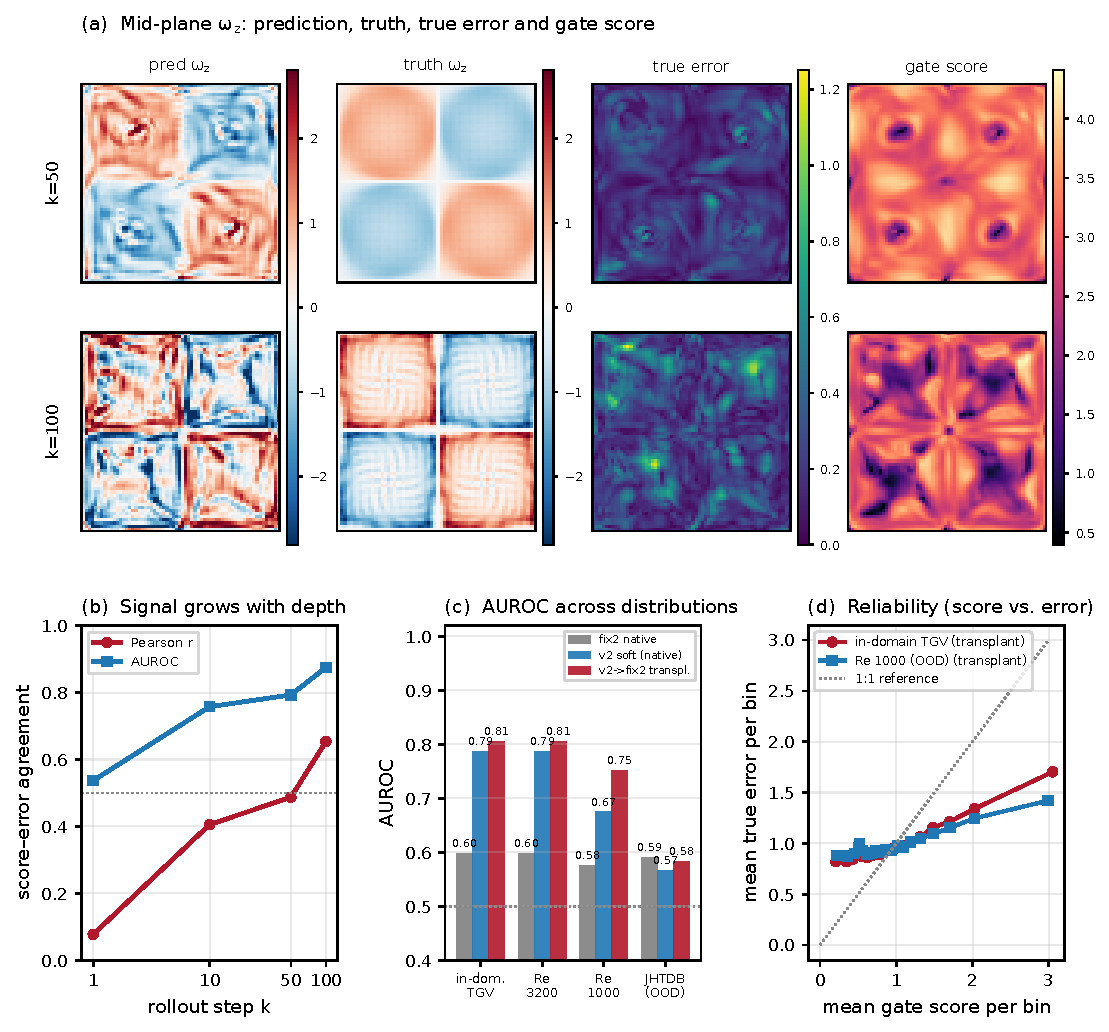
\includegraphics[width=\textwidth]{figures/fig6_upi_signal.pdf}
\caption{\textbf{Geometry-driven discrepancy indicator}. (a) Slices of the gating-signal map versus the true error map. (b) Correlation and AUROC versus horizon. (c) AUROC across distributions. (d) Calibration curve.}
\label{fig:fig6}
\end{figure}

\section{Discussion}

\subsection{Limitations and boundary conditions}

\textbf{(i) Calibration coverage}: the envelope constants must be calibrated on the target system family; when the target attractor exceeds the calibrated coverage (KS $L{=}44$), the envelope degenerates into permanent intervention (hit rate $100\%$)---it still prevents crashes but is no longer a silent safety net, and the accuracy crown of that scenario belongs to the loss-level arm. \textbf{(ii) Cross-regime transfer}: on the TGV$\to$HIT 3D regime-OOD the backbone's energy collapses ($E/E_0=0.11$ at step 1), an unsolved problem; moreover, the production term of forced turbulence is not analytically available from real-world data, which limits direct application of the envelope there. \textbf{(iii) Resolution}: the 3D main system is an under-resolved $64^3$ simulation; this does not affect the methodological conclusion on the position of physics (which holds independently on three resolution families) but limits the extrapolation of absolute accuracy claims. \textbf{(iv) Statistical robustness}: the main conclusions rest on 10 ICs with a single seed; per-IC curves are fully released, and multi-seed replication is on the supplementary agenda. \textbf{(v) Approximate reproduction}: PhysicsCorrect's official code is unavailable; the corresponding numbers carry the approximate-reproduction caveat. \textbf{(vi) Known artefact}: the envelope's delayed-release $\varepsilon(t)$ profile.

\subsection{Anatomy of the principle}

The cross-system evidence splits architecture-level physical anchoring into two independently transferable components. \emph{Hard carriage of exactly known dynamics}: accuracy gains are regime-dependent (crushing on KS in-domain, rL2 $0.015$ vs $1.18$; mainly variance contraction and short-range accuracy on 2D in-domain). \emph{Inference-path envelope}: the most robustly transferable component---silent in-domain, crash-proof at boundaries, zero-recalibration across systems and resolutions. For the general claim the latter is stronger: it relies on no fitting at all, only on the energy identity.

\subsection{Relation to structure-preserving numerical analysis}

Theorems~\ref{thm:div}--\ref{thm:gate} inherit the spirit of structure-preserving numerics: projection methods $\to$ divergence-free (Theorem~\ref{thm:div}), energy limiters $\to$ dissipation compatibility (Theorem~\ref{thm:energy}), CFL-type boundedness conditions $\to$ bounded correction (Theorem~\ref{thm:gate}). The key difference is the object being constrained: classical schemes constrain \emph{known discrete operators}, whereas we constrain \emph{a neural network with unanalysable degrees of freedom}---the guarantees must therefore be constructive and independent of network properties (projection idempotency, the scalar scaling identity). We do not claim to replace classical CFD: the target setting is rollout tasks where the true solution is unavailable and data-driven extrapolation is unavoidable; the architectural prior carries the stability ideas of classical numerical analysis into a space where no scheme exists. A point-by-point comparison table is given in SI-B.

\subsection{Methodological implications for evaluation standards}

The rL2--energy decoupling (Fig.~\ref{fig:fig7}c/d) shows that ranking long-horizon PDE rollouts by rL2 alone is systematically misleading---it rewards over-smoothing and regression to the mean. We propose three actionable reporting standards to the community: (i) comparisons at $K\ge50$ must report the energy (or corresponding invariant) trajectory and the crash rate alongside rL2; (ii) any ``zero-crash'' claim must state its crash criterion (loosen the criterion by one order of magnitude and the conclusion can flip---the data archaeology in Methods is a case in point); (iii) physics-regularised control arms should be trained with the same parameter count and curriculum as the architectural arm, otherwise the ``loss-level vs architecture-level'' conclusion is contaminated by capacity differences.

\subsection{Outlook}

(i) \textbf{Boundary mapping}: push the principle to the most complex settings (3D realistic turbulence, larger attractor dimensions) and chart the coverage and failure modes of anchor calibration---this consolidates the methodological claim more than adding yet another success case. (ii) \textbf{A PhysicsSpec catalogue}: our three systems demonstrate construction paradigms for the three families of hard-codable physics---conservation laws, linear operators, dissipation inequalities; formalising the selection criterion of \emph{which physics deserves a place on the inference path} would upgrade a point method into a design manual. (iii) \textbf{Closing the indicator loop}: feeding the discrepancy signal into adaptive time-stepping or active-learning data acquisition is a natural extension, but cross-regime calibration must be solved first.

\subsection{Answers to the editor's three questions}

(i) \emph{What general principle did we discover?} The position at which physical constraints are embedded determines the stability properties of autoregressive rollout: as a loss, physics is a suggestion; as post-processing, a patch; as an architectural prior on the inference path, a law. (ii) \emph{Which independent evidence shows it is not a single-system trick?} Three mechanistically distinct systems (3D decaying turbulence, 2D forced turbulence, 1D chaos) and six independent scenarios reproduce ``architectural anchoring beats loss-level physics'' under an isomorphic controlled protocol; a zero-parameter envelope prevents crashes across systems and resolutions with zero recalibration; three theorems provide deterministic, network-independent guarantees. (iii) \emph{When the model ``does not crash'' for a long time, is the true statistical physics also right?} Yes---energy ($1.1\%$ bias), dissipation rate, energy spectra, enstrophy and the vorticity PDF pass simultaneously; and we exhibit counter-examples (U-Net, gate90) proving that ``not crashing'' is not itself evidence of physical correctness.

\section{Conclusions}

We asked a positional question: in long-horizon neural PDE prediction, where should physical constraints live? Controlled experiments answer: on the inference path---not in the loss, not after the prediction. This positional choice changes the stability properties of rollout: zero-parameter architectural priors keep long-horizon trajectories physically feasible on three mechanistically distinct systems, while loss-level physics arms with identical parameter counts and training curricula consistently fail. Divergence-free output, dissipation compatibility and bounded correction provide deterministic guarantees independent of network internals, and the geometric discrepancy between anchor and residual emerges as a zero-cost error-diagnosis signal. The boundaries are equally clear: envelope calibration must cover the target attractor, and cross-regime transfer remains open. The next step for physical AI is not only to ``know more physics'', but to put physics where the machine cannot bypass it.

\section{Methods}

\textbf{Systems and data}. \emph{3D Taylor--Green vortex\cite{taylor1937}} at Re$=6400$: $64^3$ pseudo-spectral solver (fluidsim\cite{mohanan2019fluidsim}), 2/3 de-aliasing, $T{=}20$ long trajectories, held-out split (SPLIT\_SEED$=42$); following the grid and convergence evidence we describe this as an under-resolved pseudo-spectral simulation. \emph{2D Kolmogorov flow}: in-house vorticity--stream-function spectral solver (contour-integral ETDRK4\cite{cox2002etdrk4,kassam2005}, 2/3 de-aliasing, $\nu{=}2{\times}10^{-3}$, $A{=}0.15$, $k_f{=}4$, $\alpha{=}0.1$, $\mathrm{Re}_{\mathrm{box}}{\approx}1760$), burn-in to statistical stationarity, 14 independent initial conditions (10 train / 2 validation / 2 test); OOD sets: Re$\times2.2$, decaying turbulence and $128^2$ resolution, 3 trajectories each. \emph{1D KS}\cite{kuramoto1976,sivashinsky1977}: contour-integral ETDRK4, $L\in\{22,32,44\}$. All generators pass a one-step integration-consistency check (relative error $<10^{-6}$). JHTDB isotropic1024coarse\cite{li2008jhtdb} ($\mathrm{Re}_\lambda{=}433$) is used for OOD evaluation only, never for training.

\textbf{Data archaeology}. In the course of this study we identified and discarded two batches of legacy data: an old KS dataset that satisfies a damped variant of the equation (monotonically decaying energy, no chaos), and an old System-B dataset in which slices of a 3D field were passed off as 2D (divergence ratio $\approx1.0$, vorticity-equation residual $2$--$24$). ``Zero-crash'' conclusions once drawn on these datasets do not hold under strict criteria. Verification scripts and the deprecation record are released with the code (SI-C).

\textbf{Models and training}. \emph{3D backbone}: spectral-split hard side (Leray projection~\eqref{eq:leray} $+$ dissipation envelope~\eqref{eq:env-decay}, wired into the forward path and gradient-permeable) $+$ soft branch (3-expert spectral-convolution MoE, trained jointly with the hard side) $+$ zero-parameter calibration gate (Eqs.~\eqref{eq:gate}--\eqref{eq:fusion}) $+$ memory-bank FiLM (Supplementary Information); $5.10$M parameters; 100 epochs, AdamW $10^{-4}$ with cosine annealing, rollout$=3$ curriculum (Eq.~\eqref{eq:loss}) with scheduled sampling, one RTX 5070 Laptop GPU (8 GB), about 700 s/epoch. The hard-side bottleneck autoencoder uses spectral normalisation to maintain the Lipschitz constant (the checkable premise of Corollary~\ref{cor:bounded}). \emph{2D/1D}: the anchor is the exact linear propagator (Eqs.~\eqref{eq:ks-symbol}--\eqref{eq:phi1}; the PhysicsSpec is read from the data attributes, never hard-coded), the soft branch is an FNO2d/FNO1d (modes 12/16, width 32/64), and the three arms are parameter-matched (2D $1.19$M, 1D $0.29$M); 50 epochs with the same rollout curriculum; the full single-system experiment (including data generation) takes $<1$ hour. \emph{Implementation}: all physical operators are spectral; wavenumber grids and normalisation statistics are registered as buffers and saved with the checkpoint; on the $64^2{\to}128^2$ transfer the grid is rebuilt ($\lambda(\bm{k})$ is grid-independent---the structural basis of lossless resolution transfer); the envelope's per-step $\Delta t$ is passed from data-timestamp differences. \emph{Statistics}: mean$\pm$std across ICs; per-IC raw data released with the code. \emph{Plotting}: all figures are reproduced from the result JSONs by \texttt{scripts/make\_figures\_nc.py} in one command.

\begin{table}[htbp]
\centering\small
\caption{\textbf{Training and evaluation hyperparameters} (isomorphic protocol across the three systems; the only cross-arm variable is where the physics is placed).}
\label{tab:hyper}
\begin{tabularx}{\linewidth}{@{}>{\raggedright\arraybackslash}p{2.9cm}*{3}{>{\raggedright\arraybackslash}X}@{}}
\toprule
Item & 3D TGV (System A) & 2D Kolmogorov (B) & 1D KS (C) \\
\midrule
Grid / domain & $64^3$, $(2\pi)^3$ & $64^2$ (OOD: $128^2$), $(2\pi)^2$ & $64$, $[0,L)$, $L\in\{22,32,44\}$ \\
Viscosity / control & $\nu=1/6400$ & $\nu=2{\times}10^{-3}$, $\alpha=0.1$, $k_f=4$ & standard KS (Eq.~\eqref{eq:ks-symbol}) \\
Frame step $\Delta t$ & $0.049$ (mean, non-uniform) & $0.165$ & $0.01$ \\
Epochs / batch & 100 / 1 (accum.\ 4) & 50 / 16 & 50 / 64 \\
Optimiser / LR & AdamW $10^{-4}$ cosine & AdamW $10^{-3}$ cosine & AdamW $10^{-3}$ cosine \\
Rollout curriculum & \multicolumn{3}{c}{$R{=}3$, $\gamma_r{=}0.9$ (Eq.~\eqref{eq:loss})} \\
Envelope constants $c_d$/$c_p$ & $1.218$ / --- (decay) & $0.903$ / $0.527$ & $0.130$ / $0.130$ \\
Evaluation ICs & 10 & 5 (OOD 3) & 5 (OOD 3) \\
Crash criteria & \multicolumn{3}{c}{Table~\ref{tab:crash}, frozen filling} \\
Hardware & \multicolumn{3}{c}{Single RTX 5070 Laptop GPU (8 GB)} \\
\bottomrule
\end{tabularx}
\end{table}

\section*{Data availability}

Core custom code (architecture, training, evaluation, data generators, plotting scripts), configurations, random seeds, per-IC result JSONs and the source data for Figs.~\ref{fig:fig1}--\ref{fig:fig7} are provided with this submission. JHTDB data were obtained from the public Johns Hopkins Turbulence Database interface\cite{li2008jhtdb}. The falsification scripts and deprecation records of the data archaeology are provided alongside (Supplementary Information).
% TODO(user): upload per-IC JSONs to Zenodo and insert the DOI here before submission.

\section*{Code availability}

The full codebase is available at \url{https://github.com/chenyuze1234/rcln-pde} under the Apache 2.0 licence.

\begin{thebibliography}{99}
\footnotesize

\bibitem{li2021fno} Li, Z., Kovachki, N., Azizzadenesheli, K., Liu, B., Bhattacharya, K., Stuart, A. \& Anandkumar, A. Fourier neural operator for parametric partial differential equations. In \emph{International Conference on Learning Representations} (2021).

\bibitem{ronneberger2015} Ronneberger, O., Fischer, P. \& Brox, T. U-Net: convolutional networks for biomedical image segmentation. In \emph{Medical Image Computing and Computer-Assisted Intervention (MICCAI)}, LNCS 9351, 234--241 (2015).

\bibitem{lu2021deeponet} Lu, L., Jin, P., Pang, G., Zhang, Z. \& Karniadakis, G. E. Learning nonlinear operators via DeepONet based on the universal approximation theorem of operators. \emph{Nat. Mach. Intell.} \textbf{3}, 218--229 (2021).

\bibitem{hao2024dpot} Hao, Z., Su, C., Liu, S., Berner, J., Ying, C., Su, H., Anandkumar, A., Song, J. \& Zhu, J. DPOT: auto-regressive denoising operator transformer for large-scale PDE pre-training. In \emph{Proceedings of the 41st International Conference on Machine Learning (ICML)} (2024).

\bibitem{wu2024transolver} Wu, H., Luo, H., Wang, H., Wang, J. \& Long, M. Transolver: a fast transformer solver for PDEs on general geometries. In \emph{Proceedings of the 41st International Conference on Machine Learning (ICML)}, PMLR 235, 53681--53705 (2024).

\bibitem{kovachki2023} Kovachki, N., Li, Z., Liu, B., Azizzadenesheli, K., Bhattacharya, K., Stuart, A. \& Anandkumar, A. Neural operator: learning maps between function spaces with applications to PDEs. \emph{J. Mach. Learn. Res.} \textbf{24}(89), 1--97 (2023).

\bibitem{azizzadenesheli2024} Azizzadenesheli, K., Kovachki, N., Li, Z., Liu-Schiaffini, M., Kossaifi, J. \& Anandkumar, A. Neural operators for accelerating scientific simulations and design. \emph{Nat. Rev. Phys.} \textbf{6}, 320--328 (2024).

\bibitem{lam2023graphcast} Lam, R. et al. Learning skillful medium-range global weather forecasting. \emph{Science} \textbf{382}, 1416--1421 (2023).

\bibitem{kochkov2024neuralgcm} Kochkov, D. et al. Neural general circulation models for weather and climate. \emph{Nature} \textbf{632}, 1060--1066 (2024).

\bibitem{brandstetter2022mpnpde} Brandstetter, J., Worrall, D. E. \& Welling, M. Message passing neural PDE solvers. In \emph{International Conference on Learning Representations} (2022).

\bibitem{mccabe2023stability} McCabe, M., Harrington, P., Subramanian, S. \& Brown, J. Towards stability of autoregressive neural operators. \emph{Trans. Mach. Learn. Res.} (2023).

\bibitem{lippe2023pderefiner} Lippe, P., Veeling, B., Perdikaris, P., Turner, R. E. \& Brandstetter, J. PDE-Refiner: achieving accurate long rollouts with neural PDE solvers. In \emph{Advances in Neural Information Processing Systems 36} (2023).

\bibitem{kochkov2021mlcfd} Kochkov, D., Smith, J. A., Alieva, A., Wang, Q., Brenner, M. P. \& Hoyer, S. Machine learning--accelerated computational fluid dynamics. \emph{Proc. Natl Acad. Sci. USA} \textbf{118}(21), e2101784118 (2021).

\bibitem{raissi2019pinn} Raissi, M., Perdikaris, P. \& Karniadakis, G. E. Physics-informed neural networks: a deep learning framework for solving forward and inverse problems involving nonlinear partial differential equations. \emph{J. Comput. Phys.} \textbf{378}, 686--707 (2019).

\bibitem{li2024pino} Li, Z., Zheng, H., Kovachki, N., Jin, D., Chen, H., Liu, B., Azizzadenesheli, K. \& Anandkumar, A. Physics-informed neural operator for learning partial differential equations. \emph{ACM/IMS J. Data Sci.} \textbf{1}(3), 1--27 (2024).

\bibitem{karniadakis2021} Karniadakis, G. E., Kevrekidis, I. G., Lu, L., Perdikaris, P., Wang, S. \& Yang, L. Physics-informed machine learning. \emph{Nat. Rev. Phys.} \textbf{3}, 422--440 (2021).

\bibitem{wang2021pideeponet} Wang, S., Wang, H. \& Perdikaris, P. Learning the solution operator of parametric partial differential equations with physics-informed DeepONets. \emph{Sci. Adv.} \textbf{7}(40), eabi8605 (2021).

\bibitem{huang2025physicorrect} Huang, X. \& Perdikaris, P. PhysicsCorrect: a training-free approach for stable neural PDE simulations. \emph{Preprint at arXiv:2507.02227} (2025).

\bibitem{lee2021deepconservation} Lee, K. \& Carlberg, K. T. Deep conservation: a latent-dynamics model for exact satisfaction of physical conservation laws. \emph{Proc. AAAI Conf. Artif. Intell.} \textbf{35}(1), 277--285 (2021).

\bibitem{mohan2023hard} Mohan, A. T., Lubbers, N., Chertkov, M. \& Livescu, D. Embedding hard physical constraints in neural network coarse-graining of three-dimensional turbulence. \emph{Phys. Rev. Fluids} \textbf{8}, 014604 (2023).

\bibitem{chalapathi2024moe} Chalapathi, N., Du, Y. \& Krishnapriyan, A. Scaling physics-informed hard constraints with mixture-of-experts. \emph{Preprint at arXiv:2402.13412} (2024).

\bibitem{hairer2006gni} Hairer, E., Lubich, C. \& Wanner, G. \emph{Geometric Numerical Integration: Structure-Preserving Algorithms for Ordinary Differential Equations}, 2nd edn (Springer, 2006).

\bibitem{chorin1968} Chorin, A. J. Numerical solution of the Navier--Stokes equations. \emph{Math. Comput.} \textbf{22}, 745--762 (1968).

\bibitem{yin2021aphynity} Yin, Y. et al. Augmenting physical models with deep networks for complex dynamics forecasting. \emph{J. Stat. Mech.: Theory Exp.} \textbf{2021}, 124012 (2021).

\bibitem{gal2016dropout} Gal, Y. \& Ghahramani, Z. Dropout as a Bayesian approximation: representing model uncertainty in deep learning. In \emph{Proceedings of the 33rd International Conference on Machine Learning (ICML)}, 1050--1059 (2016).

\bibitem{lakshminarayanan2017} Lakshminarayanan, B., Pritzel, A. \& Blundell, C. Simple and scalable predictive uncertainty estimation using deep ensembles. In \emph{Advances in Neural Information Processing Systems 30} (2017).

\bibitem{yuval2020stable} Yuval, J. \& O'Gorman, P. A. Stable machine-learning parameterization of subgrid processes for climate modeling at a range of resolutions. \emph{Nat. Commun.} \textbf{11}, 3295 (2020).

\bibitem{kontolati2024latent} Kontolati, K., Goswami, S., Karniadakis, G. E. \& Shields, M. D. Learning nonlinear operators in latent spaces for real-time predictions of complex dynamics in physical systems. \emph{Nat. Commun.} \textbf{15}, 5101 (2024).

\bibitem{kuramoto1976} Kuramoto, Y. \& Tsuzuki, T. Persistent propagation of concentration waves in dissipative media far from thermal equilibrium. \emph{Prog. Theor. Phys.} \textbf{55}, 356--369 (1976).

\bibitem{sivashinsky1977} Sivashinsky, G. I. Nonlinear analysis of hydrodynamic instability in laminar flames---I. Derivation of basic equations. \emph{Acta Astronaut.} \textbf{4}, 1177--1206 (1977).

\bibitem{cox2002etdrk4} Cox, S. M. \& Matthews, P. C. Exponential time differencing for stiff systems. \emph{J. Comput. Phys.} \textbf{176}, 430--455 (2002).

\bibitem{kassam2005} Kassam, A.-K. \& Trefethen, L. N. Fourth-order time-stepping for stiff PDEs. \emph{SIAM Rev.} \textbf{47}, 631--644 (2005).

\bibitem{taylor1937} Taylor, G. I. \& Green, A. E. Mechanism of the production of small eddies from large ones. \emph{Proc. R. Soc. Lond. A} \textbf{158}, 499--521 (1937).

\bibitem{mohanan2019fluidsim} Mohanan, A. V., Bonamy, C., Linares, M. C. \& Augier, P. FluidSim: modular, object-oriented Python package for high-performance CFD simulations. \emph{J. Open Res. Softw.} \textbf{7} (2019).

\bibitem{li2008jhtdb} Li, Y. et al. A public turbulence database cluster and applications to study Lagrangian evolution of velocity increments in turbulence. \emph{J. Turbul.} \textbf{9}, N31 (2008).

\bibitem{kossaifi2024library} Kossaifi, J. et al. A library for learning neural operators. \emph{Preprint at arXiv:2412.10354} (2024).

\end{thebibliography}

\section*{Acknowledgements}
The author received no specific funding for this work.

\section*{Author contributions}
Y.C.: Conceptualization, Methodology, Software, Validation, Formal analysis, Investigation, Writing -- Original Draft, Writing -- Review \& Editing, Visualization.

\section*{Competing interests}
The author declares no competing interests.

\section*{Ethics declarations}
This work did not involve human participants, human data, or animal experiments.

\end{document}
